% !TEX program = xelatex
\PassOptionsToPackage{table}{xcolor}
\documentclass[aspectratio=169,UTF8]{ctexbeamer}

\usetheme{Madrid}
\usecolortheme{default}

\usepackage{booktabs}
\usepackage{tabularx}
\usepackage{array}
\usepackage{tikz}
\usepackage{eso-pic}
\usepackage[table]{xcolor}
\usetikzlibrary{arrows.meta,positioning,shapes.geometric}

\definecolor{ICCADBlue}{HTML}{1F4E79}
\definecolor{ICCADLightBlue}{HTML}{EAF3FA}
\definecolor{ICCADGray}{HTML}{666666}
\definecolor{ICCADLightGray}{HTML}{F4F6F8}
\definecolor{ICCADGreen}{HTML}{2E7D32}
\definecolor{ICCADOrange}{HTML}{F57C00}
\definecolor{ICCADRed}{HTML}{C62828}

\setbeamercolor{palette primary}{bg=ICCADBlue,fg=white}
\setbeamercolor{palette secondary}{bg=ICCADBlue!85,fg=white}
\setbeamercolor{palette tertiary}{bg=ICCADBlue!70,fg=white}
\setbeamercolor{frametitle}{bg=ICCADBlue,fg=white}
\setbeamercolor{title}{fg=ICCADBlue}
\setbeamerfont{frametitle}{size=\large,series=\bfseries}
\setbeamertemplate{navigation symbols}{}
\setbeamertemplate{footline}{}
\renewcommand{\arraystretch}{1.18}

\AddToShipoutPictureFG{%
  \begin{tikzpicture}[remember picture,overlay]
    \node[
      anchor=south east,
      fill=white,
      text=ICCADGray,
      minimum width=18mm,
      minimum height=5mm,
      inner sep=0pt,
      font=\scriptsize
    ] at (current page.south east) {\thepage/17};
  \end{tikzpicture}%
}

\newcommand{\key}[1]{\textcolor{ICCADBlue}{\textbf{#1}}}
\newcommand{\good}[1]{\textcolor{ICCADGreen}{\textbf{#1}}}
\newcommand{\warn}[1]{\textcolor{ICCADOrange}{\textbf{#1}}}
\newcommand{\bad}[1]{\textcolor{ICCADRed}{\textbf{#1}}}
\newcommand{\smallnote}[1]{\vspace{1mm}{\scriptsize\color{ICCADGray}#1}}

\title[Regression Failure Bucketing]{EDA 回归失败自动归因聚类期末汇报}
\subtitle{造数据、技术路线与未来思路}
\author{汇报人：李师贤}
\institute{}
\date{2026 年 6 月 16 日}

\begin{document}

% ============================================================
% 1. Title
% ============================================================
\begin{frame}[plain]
  \begin{tikzpicture}[remember picture,overlay]
    \node[
      fill=ICCADBlue,
      text=white,
      rounded corners=3pt,
      inner xsep=18pt,
      inner ysep=16pt,
      text width=0.82\paperwidth,
      align=center
    ] at (current page.center) {%
      {\LARGE\bfseries EDA 回归失败自动归因聚类期末汇报}\\[3mm]
      {\large Regression Failure Bucketing}
    };
    \node[align=center,yshift=-27mm] at (current page.center) {%
      {\normalsize 汇报人：李师贤 \quad 2026 年 6 月 16 日}\\[2mm]
      {\scriptsize\color{ICCADGray}Ibex 数据构建 + 技术路线演进 + 官方 benchmark 验证}
    };
  \end{tikzpicture}
\end{frame}

% ============================================================
% 2. 赛题任务与 BA 指标 (NEW)
% ============================================================
\begin{frame}{赛题任务与评价指标}
  \small
  \begin{columns}[T]
    \begin{column}{0.48\textwidth}
      \textbf{任务定义}
      \begin{itemize}
        \item \textbf{输入}：每个 testcase 的
        \begin{itemize}
          \item \texttt{sim.log} / \texttt{sim.log.gz} —— 仿真日志
          \item \texttt{regr.log} —— 回归比较日志
          \item \texttt{trace.log.gz} —— RISC-V 执行 trace（可选）
        \end{itemize}
        \item \textbf{输出}：\texttt{Case,bucket}
        \item \textbf{目标}：同一设计 bug（根因）的 case 分到同一桶
      \end{itemize}
    \end{column}
    \begin{column}{0.48\textwidth}
      \textbf{评价指标：Pairwise Balanced Accuracy}
      \vspace{2mm}

      {\Large \[ \mathrm{BA} = \frac{\mathrm{TPR} + \mathrm{TNR}}{2} \]}

      \vspace{2mm}
      \begin{itemize}
        \item TPR：同 bug 的 case pair 被正确分到一起的比例
        \item TNR：不同 bug 的 case pair 被正确分开的比例
        \item 同时衡量「合并质量」和「过度分裂」
      \end{itemize}
    \end{column}
  \end{columns}

  \vspace{3mm}
  \begin{center}
    \key{这是一个 pairwise 聚类问题 —— 不是简单的分类，也不是全自动聚类。}
  \end{center}
\end{frame}

% ============================================================
% 3. 核心挑战 (NEW — with real log example)
% ============================================================
\begin{frame}{核心挑战：相同症状 $\neq$ 相同根因}
  \small
  \begin{columns}[T]
    \begin{column}{0.38\textwidth}
      \textbf{为什么困难？}
      \begin{itemize}
        \item 不同 bug 可以在 sim/regr 中产生\key{高度相似}的失败签名
        \item 在当前可见特征空间中相似度极高，但官方 gold 标注为不同 bug
        \item 官方 set1 存在争议 case：同一 test 同一 seed 范围，sim/regr/trace 签名几乎无法区分，gold 却分属两个 bucket
      \end{itemize}
      \vspace{2mm}
      \textbf{这导致}
      \begin{itemize}
        \item 浅层模板匹配 → false merge（不同 bug 合并）
        \item 过于保守 → fragmentation（同一 bug 分裂成多桶）
      \end{itemize}
    \end{column}
    \begin{column}{0.58\textwidth}
      \textbf{真实案例：两 case 签名相似但 gold 不同}
      \rowcolors{2}{ICCADLightGray}{white}
      \begin{tabularx}{\linewidth}{p{2.4cm}p{2.5cm}p{2.5cm}}
        \toprule
        \textbf{维度} & \textbf{Case A (bug\_X)} & \textbf{Case B (bug\_Y)} \\
        \midrule
        regr mismatch 位置 & 0x80001000 & 0x80001000 \\
        mismatch 类型 & csr\_mstatus & csr\_mstatus \\
        sim.log 状态 & UVM TEST PASSED & UVM TEST PASSED \\
        token 集合 Jaccard & \multicolumn{2}{c}{0.94} \\
        deterministic cosine & \multicolumn{2}{c}{0.987} \\
        LLM embedding cosine & \multicolumn{2}{c}{0.952} \\
        \rowcolor{ICCADRed!15}
        \textbf{Gold bucket} & \textbf{bug\_036} & \textbf{bug\_038} \\
        \bottomrule
      \end{tabularx}
      \vspace{2mm}
      \smallnote{仅凭 sim/regr 表面信号无法区分，需要更深层的语义理解和结构化冲突信号。}
    \end{column}
  \end{columns}
\end{frame}

% ============================================================
% 4. 数据演进时间线 (compressed from 3 slides)
% ============================================================
\begin{frame}{数据演进时间线}
  \small
  \rowcolors{2}{ICCADLightGray}{white}
  \begin{tabularx}{\linewidth}{p{2.4cm}p{2.6cm}Xp{3.0cm}}
    \toprule
    \textbf{阶段（按时间）} & \textbf{规模} & \textbf{关键特征} & \textbf{作用与结论} \\
    \midrule
    1. old\_fake 三批（已废弃，Xcelium） & 80+240+640 cases，32 bugs & 期中前完成，验证全链路 & 保留为历史对照基准（first/stage2/stage3）\\
    2. VCS stage1 v1 & 40 cases，3 bugs & regr.log 仅 1 条 mismatch，无 meta.csv & 暴露格式问题，指导 v2 改进 \\
    3. stable official-like v2（当前主力） & 24 cases，4 bugs & VCS+Verdi，ibex+spike 双行对照，5 分叉点，meta.csv & \textbf{训练主力}，regr.log 格式接近官方 \\
    4. fixed official set1/set2 & 7+25 cases（Alpha 评估子集） & 官方公开 benchmark，2026-06-01 更新 & 评估迁移差距：\good{set1 BA=0.722, set2 BA=0.921} \\
    \bottomrule
  \end{tabularx}

  \vspace{3mm}
  \begin{center}
    \key{四代数据逐步逼近官方分布。v2 在 regr.log 格式上已对齐，sim.log 和失败类型仍需补强。}
  \end{center}
\end{frame}

% ============================================================
% 5. Fake vs 官方数据差异 (compressed)
% ============================================================
\begin{frame}{Fake 与官方数据的差异：指导造数据策略}
  \small
  \begin{columns}[T]
    \begin{column}{0.48\textwidth}
      \textbf{官方 benchmark 诊断发现}
      \begin{itemize}
        \item 官方同一 bug 跨 test 表现差异显著（分叉位置、失败阶段各异）
        \item debug/irq/CSR/ASSERT 信号占比高，fake 几乎纯 mismatch
        \item 官方存在争议 case：sim/regr/trace 特征高度相似但 gold 不同
        \item \textbf{结论：fake 数据失败类型过于单一}
      \end{itemize}
      \vspace{2mm}
      \textbf{v2 与官方的剩余差距}
      \begin{itemize}
        \item sim.log：v2 100\% UVM TEST PASSED；官方含 FATAL/ASSERT/timeout
        \item 失败类型：v2 仅 cosim mismatch；官方有 debug/interrupt/ASSERT
        \item 测试类型：v2 仅随机测试；官方有 directed tests
      \end{itemize}
    \end{column}
    \begin{column}{0.48\textwidth}
      \textbf{生成流程}
      \centering
      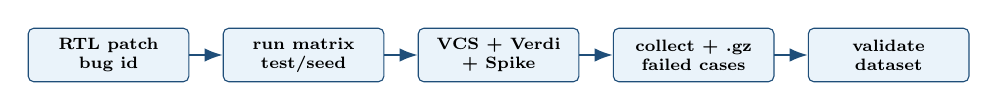
\begin{tikzpicture}[
        scale=0.85, transform shape,
        node distance=5mm,
        box/.style={draw=ICCADBlue, fill=ICCADLightBlue, rounded corners=2pt,
          minimum width=24mm, minimum height=8mm, align=center, font=\scriptsize\bfseries},
        arrow/.style={-Latex, thick, draw=ICCADBlue}
      ]
        \node[box] (patch) {RTL patch\\bug id};
        \node[box, right=of patch] (matrix) {run matrix\\test/seed};
        \node[box, right=of matrix] (vcs) {VCS + Verdi\\+ Spike};
        \node[box, right=of vcs] (collect) {collect + .gz\\failed cases};
        \node[box, right=of collect] (validate) {validate\\dataset};
        \draw[arrow] (patch) -- (matrix);
        \draw[arrow] (matrix) -- (vcs);
        \draw[arrow] (vcs) -- (collect);
        \draw[arrow] (collect) -- (validate);
      \end{tikzpicture}

      \vspace{3mm}
      \textbf{输出格式（官方兼容）}
      \begin{itemize}
        \item \texttt{case\_N/regr.log} + \texttt{sim.log.gz} + \texttt{trace.log.gz}
        \item \texttt{input.csv} + \texttt{gold.csv} + \texttt{meta.csv}
        \item 每 bug 2 tests $\times$ 3 seeds = 6 cases
      \end{itemize}
    \end{column}
  \end{columns}
\end{frame}

% ============================================================
% 6. 确定性 baseline (NEW — formal baseline flowchart)
% ============================================================
\begin{frame}{正式稳定 Baseline：确定性路线}
  \small
  \begin{center}
  \begin{tikzpicture}[
    node distance=10mm and 12mm,
    box/.style={draw=ICCADBlue, fill=ICCADLightBlue, rounded corners=2pt,
      minimum width=26mm, minimum height=9mm, align=center, font=\scriptsize\bfseries},
    arrow/.style={-Latex, thick, draw=ICCADBlue},
    label/.style={font=\fontsize{7}{8}\selectfont\color{ICCADGray}, align=center}
  ]
    \node[box] (drain) {Drain 模板\\解析};
    \node[box, right=of drain] (tfidf) {TF-IDF + SVD\\$\to$ 64d 向量};
    \node[box, right=of tfidf] (agg) {Agglomerative\\Clustering};
    \node[box, right=of agg] (output) {输出\\Case,bucket};

    \draw[arrow] (drain) -- (tfidf);
    \draw[arrow] (tfidf) -- (agg);
    \draw[arrow] (agg) -- (output);

    \node[label, below=of drain] {不依赖 LLM\\不依赖 GPU};
    \node[label, below=of tfidf] {cluster\_factor\\=0.875};
    \node[label, below=of agg] {cosine affinity\\+ ward linkage};
  \end{tikzpicture}
  \end{center}

  \vspace{3mm}
  \begin{columns}[T]
    \begin{column}{0.48\textwidth}
      \textbf{特点}
      \begin{itemize}
        \item 完全确定性，不依赖 LLM、GPU、trace.log
        \item 仅用 Drain 模板 + TF-IDF/SVD64 + Agglomerative
        \item old\_fake stage3 BA=0.779
        \item \textbf{正式预测默认方法}
      \end{itemize}
    \end{column}
    \begin{column}{0.48\textwidth}
      \textbf{明确的三层方法体系}
      \begin{enumerate}
        \item \textbf{正式 baseline}：Drain + TF-IDF/SVD + Agglomerative（确定性，默认启用）
        \item \textbf{最强实验路线}：no-trace calibrated pairwise blend（BA 0.869，experimental only）
        \item \textbf{最新架构候选}：Gated MLP（统一模型，多 seed 验证中）
      \end{enumerate}
    \end{column}
  \end{columns}
\end{frame}

% ============================================================
% 7. Pairwise Same-Bug Learning
% ============================================================
\begin{frame}{Pairwise Same-Bug Learning：从规则到学习}
  \small
  核心思路：将"直接聚类日志"转为"\key{学习两个 case 是否同源}"。指标是 pairwise BA，直接优化更有效。

  \vspace{2mm}
  \begin{columns}[T]
    \begin{column}{0.42\textwidth}
      \textbf{基础 pair 模型}
      \begin{itemize}
        \item 21d pair 特征：SVD64 cosine / 欧氏距离、token Jaccard、冲突信号
        \item 模型：Logistic / GBDT / MLP
        \item 训练：half-split，pair 采样（pos:neg=1:2），focal loss
      \end{itemize}
      \vspace{2mm}
      \textbf{5-seed half-split（3 old\_fake 数据集）}
      \rowcolors{2}{ICCADLightGray}{white}
      \begin{tabularx}{\linewidth}{p{2.3cm}p{1.3cm}p{1.3cm}p{1.3cm}}
        \toprule
        \textbf{方法} & \textbf{first} & \textbf{stage2} & \textbf{stage3} \\
        \midrule
        det (SVD64) & 0.767 & 0.745 & 0.760 \\
        pw\_logistic & 0.759 & 0.809 & 0.792 \\
        pw\_gbdt & 0.752 & \good{0.831} & \good{0.804} \\
        pw\_mlp & 0.757 & 0.828 & 0.797 \\
        \bottomrule
      \end{tabularx}
      \smallnote{pw\_gbdt mean BA=0.796（+2.2pp vs det），stage2 TNR +12pp。}
    \end{column}
    \begin{column}{0.54\textwidth}
      \textbf{LLM 双路 + 结构化特征（294 维 pair 向量）}
      \begin{itemize}
        \item 双路 LLM embedding（\texttt{features} + \texttt{summary}），各 SVD$\to$64d
        \item 14 个结构化二值信号：same\_primary\_signature、same\_mismatch\_type 等
        \item Focal loss ($\gamma$=2.0) + residual MLP
      \end{itemize}
      \vspace{1mm}
      \rowcolors{2}{ICCADLightGray}{white}
      \begin{tabularx}{\linewidth}{p{2.8cm}p{1.5cm}p{1.5cm}p{1.5cm}}
        \toprule
        \textbf{特征组合} & \textbf{first} & \textbf{stage2} & \textbf{stage3} \\
        \midrule
        LLM concat (21d) & 0.785 & 0.769 & 0.768 \\
        + structured & 0.813 & 0.819 & 0.822 \\
        + dual LLM + focal & \good{0.860} & \good{0.831} & \good{0.839} \\
        \bottomrule
      \end{tabularx}
      \vspace{2mm}
      \normalsize
      结论：\key{输入特征设计 $\gg$ 堆模型规模。dual LLM + structured 是最关键的提升。}
    \end{column}
  \end{columns}
\end{frame}

% ============================================================
% 8. Gated MLP 统一模型 (fixed — multi-seed main table)
% ============================================================
\begin{frame}{Gated MLP：期中后最大架构突破}
  \small
  \textbf{GatedResidualMLP}：在 residual backbone 前加入 feature-wise sigmoid gate + L1 正则。

  \vspace{2mm}
  \begin{columns}[T]
    \begin{column}{0.36\textwidth}
      \textbf{架构}
      \begin{itemize}
        \item 输入：294 维 pair 向量
        \item Gate：Sigmoid(gate(x)) $\times$ x + L1 正则
        \item Backbone：6 层残差 [512,512,512,256,256,128]
        \item GELU + LayerNorm + Dropout
        \item Focal Loss ($\gamma$=2.0)
      \end{itemize}
    \end{column}
    \begin{column}{0.60\textwidth}
      \textbf{7-dataset LODO 多 seed 对比}
      \rowcolors{2}{ICCADLightGray}{white}
      \begin{tabularx}{\linewidth}{p{1.7cm}p{1.5cm}p{1.5cm}p{1.5cm}p{1.5cm}}
        \toprule
        \textbf{数据集} & \textbf{Residual (0--9)} & \textbf{Gated (0--9)} & \textbf{Gated seed-0} \\
        \midrule
        first & 0.763 & \good{0.769} & 0.791 \\
        stage2 & 0.742 & \good{0.759} & 0.804 \\
        stage3 & 0.769 & \good{0.780} & 0.799 \\
        VCS off. & 0.582 & \good{0.669} & 0.743 \\
        stable & 0.481 & \good{0.563} & 0.638 \\
        set1 & 0.699 & \good{0.771} & 1.000 \\
        set2 & 0.706 & \good{0.754} & 0.917 \\
        \textbf{macro mean} & 0.677 & \good{\textbf{0.724}} & 0.813 \\
        \bottomrule
      \end{tabularx}
      \vspace{2mm}
      \smallnote{主表展示 0--9 seed 均值。seed-0 显著高于均值，set1/set2 方差大，稳定性仍需验证。}
    \end{column}
  \end{columns}
  \vspace{2mm}
  \normalsize
  \textbf{当前定位}：\key{最新统一模型候选}，全 7 域超 residual，但 inter-seed 方差大，\textbf{尚未替代正式 baseline}。
\end{frame}

% ============================================================
% 9. 交叉验证与 LODO 设计 (NEW)
% ============================================================
\begin{frame}{评估体系：交叉验证与 LODO 设计}
  \small
  \begin{columns}[T]
    \begin{column}{0.48\textwidth}
      \textbf{评估层次}
      \begin{enumerate}
        \item \textbf{half-split（5-seed）}：每个数据集内部 50/50 划分，5 个随机种子，评估 in-distribution 性能
        \item \textbf{LODO（Leave-One-Dataset-Out）}：7 个数据集轮流留一为 test，6 个训练，评估\key{跨数据分布泛化}
        \item \textbf{Official submission}：Alpha 平台盲测，评估真实迁移能力
      \end{enumerate}
      \vspace{2mm}
      \textbf{7 个评估数据集}
      \begin{itemize}
        \item 3 old\_fake：first / stage2 / stage3（保留作对照）
        \item 2 VCS fake：VCS official-like / stable official-like v2
        \item 2 官方 benchmark：fixed set1 / fixed set2
      \end{itemize}
    \end{column}
    \begin{column}{0.48\textwidth}
      \textbf{关键发现}
      \begin{itemize}
        \item old\_fake 上表现好 $\not\Rightarrow$ 官方 benchmark 上表现好
        \item set1（7 cases, k=2）和 set2（25 cases, k=4）之间也存在显著差异
        \item \textbf{domain shift 是本任务最大的泛化挑战}
        \item LODO 评估比 half-split 更能反映真实迁移性能
      \end{itemize}
      \vspace{2mm}
      \textbf{no-trace calibrated blend 的全面验证}
      \rowcolors{2}{ICCADLightGray}{white}
      \begin{tabularx}{\linewidth}{p{2.4cm}p{1.5cm}p{1.5cm}p{1.5cm}}
        \toprule
        \textbf{评估} & \textbf{seeds} & \textbf{BA} \\
        \midrule
        headline & 0--9 & \good{0.869} \\
        strict & 0--19 & \good{0.853} \\
        LODO & 7-fold & \good{0.860} \\
        \bottomrule
      \end{tabularx}
    \end{column}
  \end{columns}
\end{frame}

% ============================================================
% 10. 方法演进主结果
% ============================================================
\begin{frame}{方法演进与结果总览}
  \small
  \rowcolors{2}{ICCADLightGray}{white}
  \begin{tabularx}{\linewidth}{p{2.6cm}p{2.6cm}>{\hspace{0.5em}}Xp{2.0cm}}
    \toprule
    \textbf{阶段} & \textbf{做法} & \textbf{核心结论} & \textbf{BA 提升} \\
    \midrule
    Baseline & Drain+TF-IDF/SVD64+Agglomerative & 稳定但仅用浅层模板 & 0.779 \\
    Pairwise 建模 & 21d pair + GBDT/MLP & 学习 P(same\_bug)，超 concat & +2.2pp \\
    LLM Embedding & Nomic 768d + SVD64 拼接 & stage2 TNR 0.744$\to$0.788 & +4.4pp TNR \\
    Dual LLM+Struct & 双路 LLM + structured signals + focal MLP & 输入设计 $\gg$ 堆模型 & +5.1pp \\
    Calibrated Blend & $\alpha$=0.88, rt=1.15, et=1.00 & 0--9 mean BA=\good{0.869} & — \\
    Gated MLP & sigmoid gate + 6 层残差 + L1 & 全 7 fold 超 residual（+4.7pp） & +12.5pp (s0) \\
    Bridge-Edge & OOF 识别分片桥接边 $\to$ 辅助 loss & 好种子 BA$\sim$0.91，坏种子崩溃 & 不稳定 \\
    Trace/Completion & 52d trace / completion evidence & VCS +5.2\%，set2 $-$8.1\% & 域依赖 \\
    \bottomrule
  \end{tabularx}

  \vspace{3mm}
  \begin{center}
    \key{当前最强实验路线：no-trace calibrated blend（BA 0.869）。Gated MLP 是下一步 backbone 候选。}
  \end{center}
\end{frame}

% ============================================================
% 11. 官方 set1/set2 结果 (with case count clarification)
% ============================================================
\begin{frame}{官方 Benchmark 验证与 Alpha 提交}
  \small
  \begin{columns}[T]
    \begin{column}{0.48\textwidth}
      \textbf{Alpha 提交（2026-06-06）}
      \begin{itemize}
        \item 方法：no-trace calibrated dual-input blend
        \begin{itemize}
          \item $\alpha$=0.88, rich\_temp=1.15, ensemble\_temp=1.00
          \item logistic 0.20 + GBDT 0.40 + MLP 0.40
        \end{itemize}
      \end{itemize}
      \rowcolors{2}{ICCADLightGray}{white}
      \begin{tabularx}{\linewidth}{p{1.8cm}p{1.4cm}p{1.4cm}p{1.4cm}p{1.2cm}}
        \toprule
        \textbf{数据集} & \textbf{BA} & \textbf{TPR} & \textbf{TNR} & \textbf{耗时} \\
        \midrule
        set1 (7 cases, k=2) & \good{0.722} & 0.778 & 0.667 & 5.1s \\
        set2 (25 cases, k=4) & \good{0.921} & 0.957 & 0.885 & 9.4s \\
        \bottomrule
      \end{tabularx}
      \vspace{2mm}
      \smallnote{Alpha 评估子集：7 / 25 valid cases（过滤后有效 case 数）。时限 90s，均大幅低于上限。}

      \vspace{3mm}
      \textbf{关键启示}
      \begin{itemize}
        \item set1 $\ll$ set2：小样本 + 跨 bug 相似度高 → 泛化困难
        \item set1 的 0.722 说明\bad{当前方法对小样本跨域场景仍不足}
      \end{itemize}
    \end{column}
    \begin{column}{0.48\textwidth}
      \textbf{set1 失败案例分析}
      \begin{itemize}
        \item set1 仅 7 cases，2 bucket，但 case 间签名高度相似
        \item 存在同一 test、同一 seed 范围、sim/regr/trace 特征近乎一致的 case pair，gold 标注为不同 bug
        \item 当前模型在这些「争议 case」上的概率接近 0.5，无法可靠区分
      \end{itemize}
      \vspace{2mm}
      \textbf{这验证了核心挑战}
      \begin{enumerate}
        \item 表面日志相似 $\neq$ 同根因 —— 需要更深层语义
        \item 小样本场景需要更强的先验或对比学习
        \item 争议 case 本身可能是官方标注粒度的差异
      \end{enumerate}
    \end{column}
  \end{columns}
\end{frame}

% ============================================================
% 12. Trace/Completion 消融与失败经验 (compressed)
% ============================================================
\begin{frame}{Trace 与 Completion 路线：尝试与经验}
  \small
  \begin{columns}[T]
    \begin{column}{0.48\textwidth}
      \textbf{Trace 路线：有信号但不稳定}
      \rowcolors{2}{ICCADLightGray}{white}
      \begin{tabularx}{\linewidth}{p{1.8cm}p{1.8cm}p{1.8cm}}
        \toprule
        \textbf{实验} & \textbf{正向} & \textbf{反向} \\
        \midrule
        Route A 52d 特征 & VCS +5.2\% BA & set2 $-$8.1\% \\
        Modality Dropout & first+5.9\%, stage2+4.5\% & set1 $-$47.2\% \\
        Anchor w64 (同数据集诊断) & \textcolor{ICCADGray}{BA=0.984}\textsuperscript{*} & no\_trace 0.590 \\
        \bottomrule
      \end{tabularx}
      \vspace{1mm}
      \smallnote{*Anchor w64 BA=0.984 是\bad{同数据集训练+评估的诊断结果}，\\
      仅证明 trace 中存在强信号，\bad{不代表未见数据泛化能力}。}

      \vspace{2mm}
      \textbf{Completion 路线：证据抽取器}
      \begin{itemize}
        \item 不直接输出 bucket，只输出 canonical evidence JSON
        \item 白名单枚举太粗 → false merge 增加
        \item 第一轮 structured-completion 未超 base
      \end{itemize}
    \end{column}
    \begin{column}{0.48\textwidth}
      \textbf{共同经验}
      \begin{enumerate}
        \item 额外信号（trace/completion）\key{有信息量}，但\bad{随数据集漂移}
        \item 不能作为全局默认特征，需要\key{conditional gating}
        \item 正确的方向：\key{validation-trained pair-level gating} + \key{selective expert routing}
        \item 模型不应知道数据来源（source identity），gate 从 held-out validation pairs 学习
      \end{enumerate}
      \vspace{2mm}
      \textbf{当前定位}
      \begin{itemize}
        \item Trace：\warn{保留为事后复核/诊断工具}
        \item Completion：\warn{管线已通，gate 调优中}
        \item 两者均\bad{不默认启用}，统一为 selective expert evidence
      \end{itemize}
    \end{column}
  \end{columns}
\end{frame}

% ============================================================
% 13. 工程交付 (NEW)
% ============================================================
\begin{frame}{工程交付：从实验到可用系统}
  \small
  \begin{columns}[T]
    \begin{column}{0.48\textwidth}
      \textbf{接口与兼容性}
      \begin{itemize}
        \item 正式预测接口：\texttt{regr\_fail\_bucketing.py}
        \item 输入：\texttt{input.csv}（Case, Regr Log, Sim Log, Trace Log）
        \item 输出：\texttt{Case,bucket}
        \item 支持 \texttt{.gz} 压缩日志透明读取
        \item 缺 trace 文件时 graceful fallback（zero embedding）
      \end{itemize}
      \vspace{2mm}
      \textbf{运行时性能}
      \begin{itemize}
        \item Alpha 提交：set1 5.1s / set2 9.4s，均远低于 90s 时限
        \item LLM embedding 缓存：避免重复 API 调用
        \item GPU 推理 batch size 100k pairs，支持百 case 规模
      \end{itemize}
    \end{column}
    \begin{column}{0.48\textwidth}
      \textbf{确定性保证}
      \begin{itemize}
        \item 正式默认方法（Drain + SVD + Agglomerative）完全确定性
        \item 所有实验方法通过 seed 参数控制可复现性
        \item LLM 仅用于 embedding，不调用 completion（正式预测）
      \end{itemize}
      \vspace{2mm}
      \textbf{关键约束（始终遵守）}
      \begin{itemize}
        \item 正式预测不读取 gold.csv 或 meta.csv
        \item 默认不使用 trace.log
        \item LLM 只用于 embedding，不调用 completion
        \item 缺文件时 graceful fallback，不阻断管线
      \end{itemize}
    \end{column}
  \end{columns}
\end{frame}

% ============================================================
% 14. 数据 v2→v3 规划 (compressed from future pages)
% ============================================================
\begin{frame}{下一步：数据 v3 与架构演进}
  \small
  \begin{columns}[T]
    \begin{column}{0.48\textwidth}
      \textbf{数据 v3 规划（P0）}
      \begin{itemize}
        \item 补齐失败类型：debug timeout、interrupt timeout、ASSERT、FAILED（非 mismatch）
        \item 引入 directed tests（debug\_basic\_test 等）
        \item 构造同一 bug 跨 mismatch 与 FAILED 的混合 case
        \item 目标：失败类型分布对齐官方 benchmark
      \end{itemize}
      \vspace{2mm}
      \textbf{架构演进（P0）}
      \begin{itemize}
        \item Gated MLP 完成 0--9 seed 稳定性验证 + inner calibration
        \item 替代 residual 成为新 backbone 候选
        \item Completion selective expert gate 调优 + teacher distillation
      \end{itemize}
    \end{column}
    \begin{column}{0.48\textwidth}
      \textbf{Selective Expert 完善（P1）}
      \begin{itemize}
        \item Bridge-Edge Mining 稳定化：multi-seed OOF ensemble + quality gate
        \item Trace/Completion 统一为 validation-trained pair-level gating
        \item 专家不可用时 gate 权重严格为 0，不破坏 base 结果
      \end{itemize}
      \vspace{2mm}
      \textbf{评估对齐（P1）}
      \begin{itemize}
        \item 7-dataset LODO 持续评估
        \item 对齐 B\_20260601 新 benchmark 规则
        \item 跨域泛化：fake $\to$ official 迁移差距持续监控
      \end{itemize}
    \end{column}
  \end{columns}

  \vspace{3mm}
  \begin{center}
    \key{四条主线：数据 $\to$ 架构 $\to$ 证据 $\to$ 评估。目标：让模型在未见 bug 类型上也能可靠聚类。}
  \end{center}
\end{frame}

% ============================================================
% 15. 核心贡献与局限
% ============================================================
\begin{frame}{核心贡献与局限}
  \large
  \textbf{已完成的工作}

  \vspace{3mm}
  \small
  \renewcommand{\arraystretch}{1.45}
  \begin{tabularx}{0.95\linewidth}{p{3.4cm}X}
    \toprule
    \textbf{数据建设} & official-format v1$\to$v2 两版迭代（VCS 工具链），gold.csv + .gz 压缩，regr.log 含 ibex+spike 双行对照；四代数据逐步逼近官方分布。\\
    \midrule
    \textbf{方法演进} & 从 Drain+Agglomerative（BA 0.779）到 no-trace calibrated blend（BA 0.869），pairwise learning + dual LLM + structured features + focal loss 逐级提升。\\
    \midrule
    \textbf{架构创新} & Gated MLP 在 7-dataset LODO 全胜 residual（macro BA 0.724 vs 0.677），作为下一代 backbone 候选。\\
    \midrule
    \textbf{工程系统} & 确定性 baseline + 实验 blend + selective expert 三层体系；gzip 透明读取、LLM 缓存、graceful fallback、Alpha 提交通过。\\
    \midrule
    \textbf{诚实记录} & Trace/Completion/Bridge-Edge 等失败路线如实记录分析，不 cherry-pick 结果。Domain shift 问题充分暴露。\\
    \bottomrule
  \end{tabularx}
  \renewcommand{\arraystretch}{1.18}

  \vspace{2mm}
  \textbf{主要局限}
  \begin{itemize}
    \item v2 数据失败类型仍单一（缺 FAILED/FATAL/ASSERT），与官方分布有差距
    \item set1 小样本场景（7 cases）BA 仅 0.722，跨域泛化仍不足
    \item Gated MLP inter-seed 方差大，尚未稳定到可以替代正式 baseline
    \item Selective expert gate 调优仍处于早期阶段
  \end{itemize}
\end{frame}

% ============================================================
% 16. 下一步与 小组组员分工
% ============================================================
\begin{frame}{下一步计划}
  \small
  \begin{columns}[T]
    \begin{column}{0.48\textwidth}
      \textbf{短期（考试结束后 $\sim$ 2 周）}
      \begin{enumerate}
        \item \key{Gated MLP 0--9 seed 稳定性验证 + inner calibration}
        \item \key{数据 v3 制造：补齐 FAILED/FATAL/ASSERT + directed tests}
        \item Completion selective expert gate 调优
        \item Bridge-Edge multi-seed ensemble 稳定化
      \end{enumerate}
      \vspace{2mm}
      \textbf{中期（$\sim$ 4 周）}
      \begin{enumerate}
        \item Gated MLP 替代 residual 成为新 backbone
        \item 7-dataset LODO 全面验证 + 对齐新 benchmark 规则
        \item Selective expert 框架完成第一版集成
      \end{enumerate}
    \end{column}
    \begin{column}{0.48\textwidth}
      \textbf{长期目标（$\sim$ 8 周）}
      \begin{enumerate}
        \item 确定性 baseline + Gated MLP + selective expert 三层体系稳定
        \item set1-level 小样本场景 BA 目标 $\ge$ 0.85
        \item 正式预测方案锁定
      \end{enumerate}

      \vspace{3mm}
      {\color{ICCADBlue}\hrule}
      \vspace{3mm}
      \textbf{小组组员分工}
      \begin{itemize}
        \item 李师贤：算法设计与模型训练、数据制造、实验评估
        \item [组员 2]：[分工待补充]
        \item [组员 3]：[分工待补充]
      \end{itemize}
    \end{column}
  \end{columns}
\end{frame}

% ============================================================
% 17. Thank you
% ============================================================
\begin{frame}[plain]
  \begin{tikzpicture}[remember picture,overlay]
    \fill[ICCADLightBlue] (current page.south west) rectangle (current page.north east);
    \node[text=ICCADBlue, font=\fontsize{36}{44}\selectfont\bfseries]
      at (current page.center) {谢谢！};
    \node[align=center,yshift=-16mm] at (current page.center) {%
      {\normalsize\color{ICCADGray}EDA 回归失败自动归因聚类}\\[2mm]
      {\small\color{ICCADGray}ICCAD 2026 Problem B}
    };
  \end{tikzpicture}
\end{frame}

\end{document}
